\section{Introducción}

El objetivo de este Trabajo Práctico es simular las tiradas de 3 monedas, de las cuales 1 está cargada (aunque se ignora cómo), y en base a un modelo ha construir y los datos de las tiradas que se realizaron,
inferir cuál de las 3 monedas es la cargada, y qué tan cargada esta. A continuación el enunciado:

~\\
\textbf{Observamos 10 tiradas de 3 monedas distintas, de las que sabemos que hay dos monedas comunes y una cargada, aunque ignoramos cargada cómo. Los números de caras obtenidos para las distintas
monedas en las 10 tiradas son 3, 4 y 10.}


\section{Problema 1: Modelo y Representación Gráfica}

\textbf{Escriba un modelo que capture el problema enunciado. Realice una representación gráfica del modelo propuesto, utilizando la convención para identificar
nodos latentes, observados y deterministicos.}


%IMAGEN
\begin{minipage}[t]{\dimexpr\linewidth-5.5cm\relax}
    \raggedleft\raisebox{\dimexpr 0.6\baselineskip-\height}{
    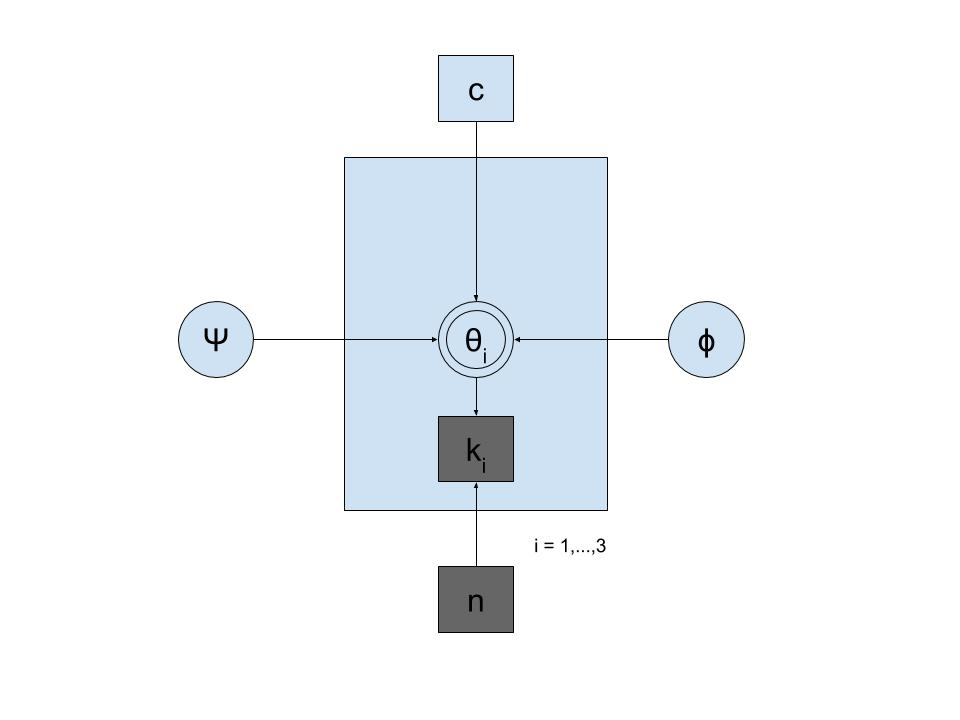
\includegraphics[width=\textwidth]{imagenes/modelo1.jpg}}
    \captionof{figure}{\texttt{modelo 1}}
\end{minipage}\hfill
%TEXTO AL LADO
\begin{minipage}[t]{0.7\textwidth}
  \begin{flushleft}
  \large
    ~\\
    $\Psi \; {\raise.17ex\hbox{$\scriptstyle\sim$}} \; Beta(1000, 1000)$\vspace*{0.3cm} \\
    $\Phi \; {\raise.17ex\hbox{$\scriptstyle\sim$}} \; Beta(1,1)$\vspace*{0.3cm} \\
    $\Theta_{i} = \left\{
	  \begin{array}{ll}
		  \Phi  & \mbox{si } c = i \\
		  \Psi & \mbox{si } c \neq i
	  \end{array}
    \right.$\vspace*{0.3cm} \\
    $C \; {\raise.17ex\hbox{$\scriptstyle\sim$}} \; Categorical(1/3,1/3,1/3)$\vspace*{0.3cm} \\
    $K_{i} \; {\raise.17ex\hbox{$\scriptstyle\sim$}} \; Binomial(n, \theta_{i})$  
  \end{flushleft}  
\end{minipage}

~\\ \\

Donde $\Phi$ representa el prior de la moneda cargada (Uniforme(0,1) ya que no se sabe cómo esta cargada) y $\Psi$ el prior para las monedas no cargadas, el cual elegí representarlo
como una Beta(1000, 1000), para que la función esté lo más concentrada posible alrededor de $1/2$, como se puede observar en la Figura 2. Por último, $\Theta_{i}$ es igual a $\Phi$ o $\Psi$ según
el resultado de la categórica $C$, que decide cuál de las 3 monedas es la cargada, y $K_{i}$ es la binomial que representa la cantidad de caras obtenidas por cada moneda luego de 10 tiradas.

\begin{figure}[h!]
  \centering
    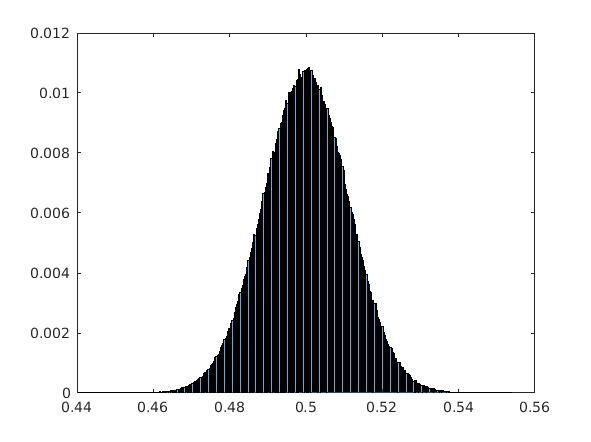
\includegraphics[width=0.5\textwidth]{imagenes/beta-1000-1000.jpg}
  \caption{Beta(1000,1000)}
\end{figure}


\newpage
El modelo en JAGS es el siguiente:
\begin{verbatim}
model{
   #m = cantidad de monedas

   for (i in 1:m) {
   		p[i] = 1/3
   }
   #Priors
   c ~ dcat(p[])
   phi ~ dbeta(1,1) #cargada, pero no se como
   psi ~ dbeta(1000,1000) #no cargada, quiero que este lo mas concentrado posible en 1/2

   for (i in 1:m) {
   		theta[i] <- equals(c[1], i)*phi + (1 - equals(c[1], i))*psi
   		k[i] ~ dbin(theta[i], n)
   }
}
\end{verbatim}

\newpage
\section{Problema 2: Implementación e Inferencia}

\textbf{Implemente el modelo en su sistema de inferencia predilecto, y obtenga muestras de la posterior para las variables relevantes. Explicite cuáles fueron los parámetros
elegidos para el algoritmo de muestreo.}

\begin{itemize}
 \item \textbf{\textit{Realice histogramas de las distintas variables, utilizando un mismo gráfico cuando sea posible/razonable.}}
 \item \textbf{\textit{Reporte la media y el desvío estándar para todas las variables inferidas.}}
 \item \textbf{\textit{Compute la probabilidad a posteriori de que cada una de las monedas sea la moneda cargada.}}
\end{itemize}


Para implementar este modelo utilizé \textit{MatJAGS} junto con Matlab R2016a. Las variables relevantes a muestrear son $C$ (qué moneda es la cargada) y los distintos $\Theta$ (la probabilidad
de salir cara de cada moneda). Los parámetros para el algoritmo de muestreo son: 

\begin{itemize}
 \item \textit{nchains = 2} (cantidad de cadenas)
 \item \textit{nburnin = 100} (burn-in examples)
 \item \textit{nsamples = 5000} (cant. de samples)
 \item \textit{thin = 2} (cada cuánto sampleo)
\end{itemize}

Los histogramas para cada una de las variables de interes son los siguientes:


\begin{figure}[h!]
  \centering
    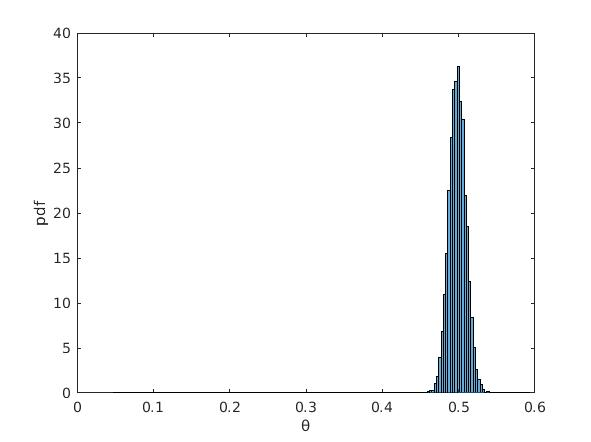
\includegraphics[width=0.6\textwidth]{imagenes/theta1.jpg}
  \caption{theta 1}
\end{figure}

Con media = 0.4975 y std = 0.0190

\newpage 

\begin{figure}[h]
    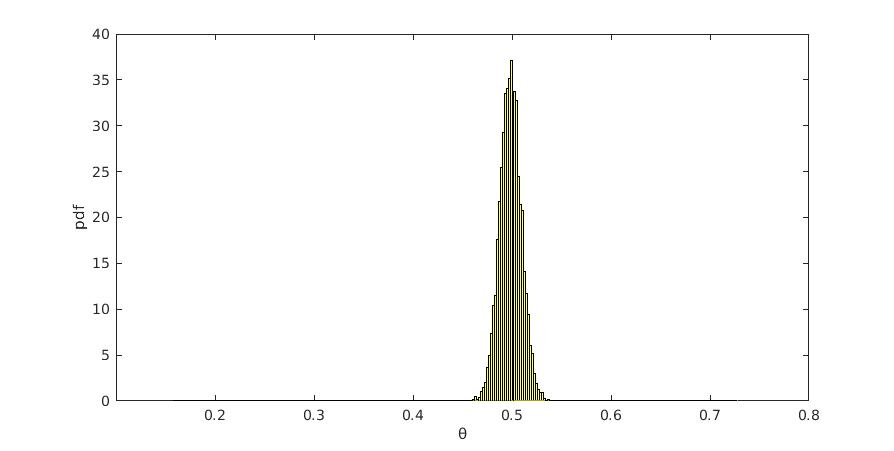
\includegraphics[width=0.9\textwidth]{imagenes/theta2.jpg}
  \caption{theta 2}
\end{figure}

Con media = 0.4981 y std = 0.0152

~\\
\begin{figure}[h]
    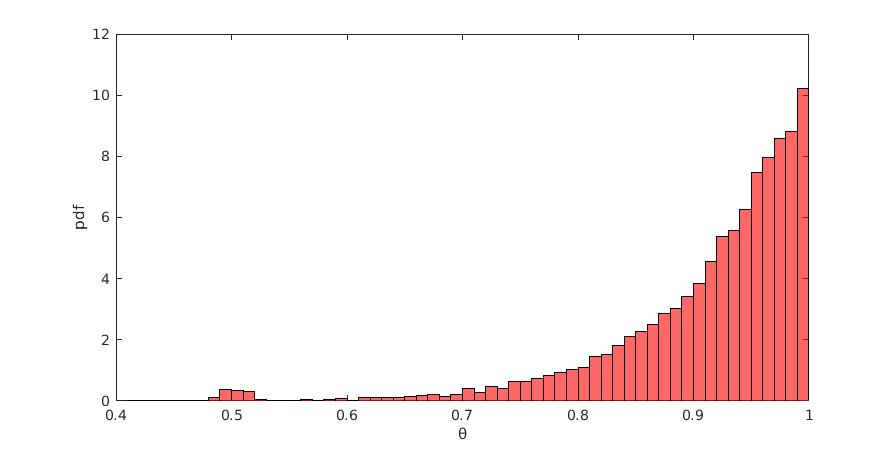
\includegraphics[width=0.9\textwidth]{imagenes/theta3.jpg}
  \caption{theta 3}
\end{figure}

Con media = 0.9131 y std = 0.0866

\newpage

Las diferencias y similitudes entre las posterior de los $\Theta$ de cada moneda se pueden apreciar mejor en el siguiente gráfico conjunto:

~\\
\begin{figure}[h]
    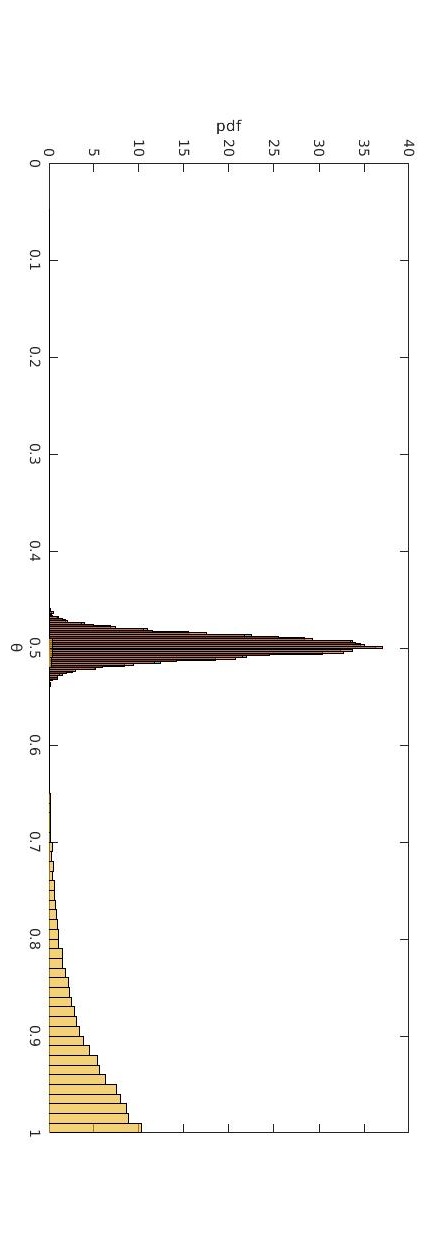
\includegraphics[width=0.4\textwidth]{imagenes/conjunta.jpg}
  \caption{theta 1, 2, y 3}
\end{figure}
~\\

Se puede ver que $\Theta_{1}$ y $\Theta_{2}$ están prácticamente solapados con media alrededor de $0.5$, mientras que $\Theta_{3}$, como resultó ser la moneda cargada, tiene una
distribución con mucho peso en valores cercanos al $1$, similar a una $Beta(1000,1)$.	

\newpage

En cuanto a la variable categórica $C$, podemos observar su resultado en el siguiente gráfico:

~\\
\begin{figure}[h]
    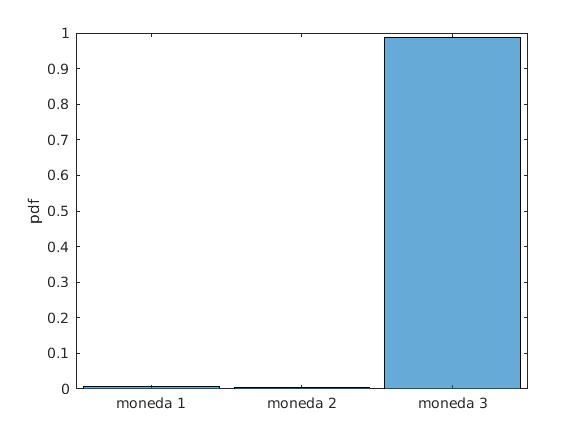
\includegraphics[width=0.8\textwidth]{imagenes/categorica.jpg}
  \caption{categórica}
\end{figure}
~\\

De donde se puede ver claramente que la probabilidad de que la tercera moneda sea la cargada es prácticamente $1$, mientras que la probabilidad de que las monedas 1 y 2 sean las
cargadas es muy cercana a $0$.



\newpage

\section{Problema 3: Modificaciones al Modelo}

\textbf{Discuta cómo modificaría el modelo si en lugar de saber que hay una moneda cargada, nos dicen que cada moneda puede estar cargada o no con probabilidad 1/2 independientemente
de las otras monedas. Provea el modelo y su representación gráfica para este caso.}

~\\
La modificación que hay que realizarle al modelo es sencilla: la variable categórica $C$ se reemplaza por 3 variables bernoulli $C_{1}$, $C_{2}$ y $C_{3}$ con parámetro $1/2$ (una para cada $\Theta$),
las cuales deciden para cada moneda si ésta va a estar cargada o no. La representación gráfica de este modelo se puede ver en la siguiente Figura:

%IMAGEN
\begin{minipage}[t]{\dimexpr\linewidth-5.5cm\relax}
    \raggedleft\raisebox{\dimexpr 0.6\baselineskip-\height}{
    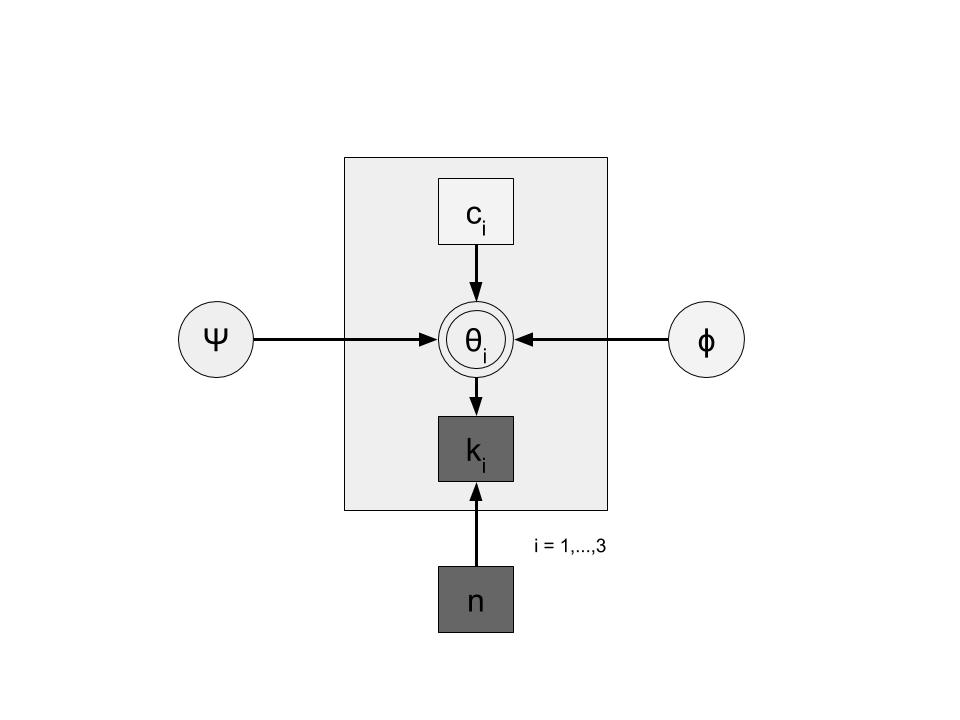
\includegraphics[width=\textwidth]{imagenes/modelo2.jpg}}
    \captionof{figure}{\texttt{modelo 2}}
\end{minipage}\hfill
%TEXTO AL LADO
\begin{minipage}[t]{0.7\textwidth}
  \begin{flushleft}
  \large
    ~\\
    $\Psi \; {\raise.17ex\hbox{$\scriptstyle\sim$}} \; Beta(1000, 1000)$\vspace*{0.3cm} \\
    $\Phi \; {\raise.17ex\hbox{$\scriptstyle\sim$}} \; Beta(1,1)$\vspace*{0.3cm} \\
    $\Theta_{i} = \left\{
	  \begin{array}{ll}
		  \Phi  & \mbox{si } c = i \\
		  \Psi & \mbox{si } c \neq i
	  \end{array}
    \right.$\vspace*{0.3cm} \\
    $C \; {\raise.17ex\hbox{$\scriptstyle\sim$}} \; Bernoulli(1/2)$\vspace*{0.3cm} \\
    $K_{i} \; {\raise.17ex\hbox{$\scriptstyle\sim$}} \; Binomial(n, \theta_{i})$  
  \end{flushleft}  
\end{minipage}

~\\ \\

El modelo en JAGS es el siguiente:

\begin{verbatim}
model{
   #m = cantidad de monedas

   #Priors
   for (i in 1:m) {
   	   c[i] ~ dbern(0.5)
   }
   
   phi ~ dbeta(1,1) #cargada, pero no se como
   psi ~ dbeta(1000,1000) #no cargada, quiero que este lo mas concentrado posible en 1/2

   for (i in 1:m) {
   		theta[i] <- equals(c[i], 1)*phi + equals(c[i], 0)*psi
   		k[i] ~ dbin(theta[i], n)
   }
}
\end{verbatim}

~\\
\newpage
En este caso el histograma para las posterior de las variables $\Theta$ es:

\begin{figure}[h]
    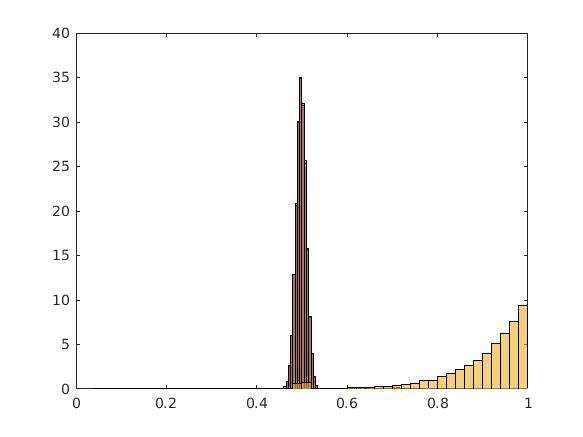
\includegraphics[width=0.9\textwidth]{imagenes/conjunta-modelo2.jpg}
  \caption{theta 1, 2, y 3}
\end{figure}
~\\

Con las siguientes medias y desvíos estándar:

~\\

$\Theta_{1} = 0.4980, 0.0298$ (incremento del 1\% y 1.57\% en media y std con respecto al modelo anterior)

$\Theta_{2} = 0.5002, 0.0321$ (incremento del 1\% y 2.11\% en media y std con respecto al modelo anterior)

$\Theta_{3} = 0.8986, 0.1091$ (decremento del 1\% en media e incremento del 1.26\% en std con respecto al modelo anterior)


~\\
Y los diagramas para las posterior de las categóricas $C_{i}$ son los siguientes, en los cuales se puede 
observar que la moneda 3 es la cargada.


\begin{figure}[h!]
  \centering{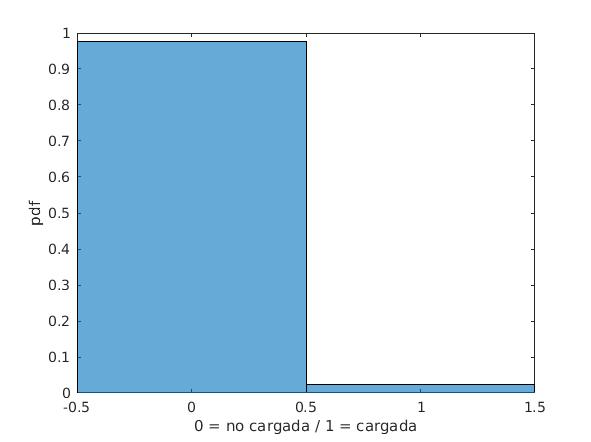
\includegraphics[width=0.5\textwidth]{imagenes/c1.jpg}}
  \caption{c1}
\end{figure}

\begin{figure}[h!]
  \centering{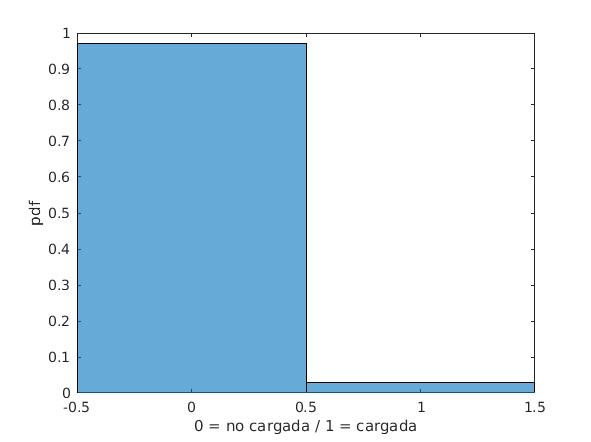
\includegraphics[width=0.5\textwidth]{imagenes/c2.jpg}}
  \caption{c2}
\end{figure}

\begin{figure}[h!]
  \centering{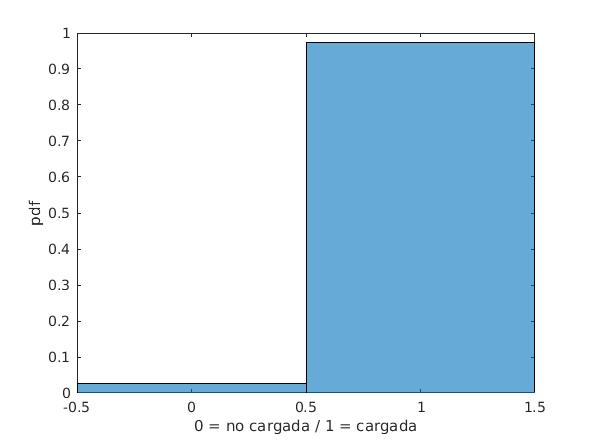
\includegraphics[width=0.5\textwidth]{imagenes/c3.jpg}}
  \caption{c3}
\end{figure}


\clearpage

\section{Problema 4: Predicciones}

\textbf{Escriba la expresión para la probabilidad de obtener cara en la próxima tirada para cada una de las monedas. 
¿Qué distintas fuentes de incertidumbre puede identificar en ella?}

La expresión para la probabilidad de obtener cara en la próxima tirada es la posterior predictive de la moneda, la cual tiene la siguiente forma:

~\\
{\Large
${\displaystyle \int} P(cara | D,c) = {\displaystyle \int} P(cara, \Theta_{i} | D, c) \; d\Theta_{i} = {\displaystyle \int} P(cara | \Theta_{i}, D, c) \ P(\Theta_{i} | D, c) \; d\Theta_{i} =
{\displaystyle \int} P(cara | \Theta_{i}) \ P(\Theta_{i} | D, c) \; d\Theta_{i} = {\displaystyle \int} P(cara | \Theta_{i}) \ [ P(\Phi | D) I(c = i) \ + \ P(\Psi | D) I(c \neq i)] \; d\Theta_{i} = 
{\displaystyle \int} P(cara | \Theta_{i}) \ [ P(\Phi) I(c = i) \ + \ P(\Psi) I(c \neq i)] \; d\Theta_{i}$

}

~\\

Una fuente de incertidumbre es el valor real de la categórica $C$, que determina cual de las 2 distribuciones voy a terminar usando para calcular la posterior predictive.

\newpage
\section{Apéndice: Código matlab}

El código a continuación es todo el código utilizado en el tp:

\begin{verbatim}
%% TP

clear;
modelo = 2; %1 = primer model, 2 = modelo modificado

modelo_txt = '';

if modelo == 1
    modelo_txt = 'model.txt';
else
    modelo_txt = 'model2.txt';
end

%% Data (Observed Variables)
k = [3, 4, 10];
n = 10;
m = 3; %cantidad de monedas

%% Sampling
% MCMC Parameters
nchains = 2; % How Many Chains?
nburnin = 1e2; % How Many Burn-in Samples?
nsamples = 5e3;  %How Many Recorded Samples?
nthin = 2; % How Often is a Sample Recorded?
doparallel = 0; % Parallel Option

% Assign Matlab Variables to the Observed Nodes
datastruct = struct('k', k, 'n', n, 'm', m);

%Initialize Unobserved Variables
for i=1:nchains
    if modelo == 1
        S.c = 1/3;
    else
        S.c = round(rand(1,m));
    end
        
    init0(i) = S;
end


% Use JAGS to Sample
tic
fprintf( 'Running JAGS ...\n' );
[samples, stats] = matjags( ...
	datastruct, ...
	fullfile(pwd, modelo_txt), ...
	init0, ...
	'doparallel' , doparallel, ...
	'nchains', nchains,...
	'nburnin', nburnin,...
	'nsamples', nsamples, ...
	'thin', nthin, ...
	'monitorparams', {'c', 'theta'}, ...
	'savejagsoutput' , 1 , ...
	'verbosity' , 1 , ...
	'cleanup' , 0 , ...
	'workingdir' , 'tmpjags' );
toc

%Grafico los resultados

theta1 = samples.theta(:,:,1);
theta2 = samples.theta(:,:,2);
theta3 = samples.theta(:,:,3);
theta1 = theta1(:);
theta2 = theta2(:);
theta3 = theta3(:);

if modelo == 1
    c = samples.c();
    c = c(:);

    %a = ordinal(c, {'moneda 1', 'moneda 2', 'moneda 3'});
    %histogram(a, 'Normalization', 'pdf');

    %histogram(theta1, 'Normalization', 'pdf');
    %hold on
    %histogram(theta2, 'Normalization', 'pdf');
    %hold on
    %histogram(theta3, 'Normalization', 'pdf');
else
    c1 = samples.c(:,:,1);
    c2 = samples.c(:,:,2);
    c3 = samples.c(:,:,3);
    c1 = c1(:);
    c2 = c2(:);
    c3 = c3(:);
    
    
    %histogram(theta1, 'Normalization', 'pdf');
    %hold on
    %histogram(theta2, 'Normalization', 'pdf');
    %hold on
    %histogram(theta3, 'Normalization', 'pdf');
    %histogram(c1, 'Normalization', 'pdf');
    %histogram(c2, 'Normalization', 'pdf');
    %histogram(c3, 'Normalization', 'pdf');
end
 

 

\end{verbatim}
